\documentclass[aps,pra,reprint,superscriptaddress,nofootinbib,longbibliography]{revtex4-2}

\usepackage{cmap}
\usepackage[utf8]{inputenc}
\usepackage[T1]{fontenc}
\usepackage{amsmath,amssymb,amsthm}
\usepackage{mathtools}
\usepackage{graphicx}
\usepackage{hyperref}
\usepackage{xcolor}
\usepackage{bm}

%------------------------------------------------
% theorem environments
%------------------------------------------------

\newtheorem{theorem}{Theorem}[section]
\newtheorem{lemma}[theorem]{Lemma}
\newtheorem{proposition}[theorem]{Proposition}
\newtheorem{corollary}[theorem]{Corollary}
\newtheorem{definition}[theorem]{Definition}
\newtheorem{remark}[theorem]{Remark}
\newtheorem{openproblem}[theorem]{Open Problem}

%------------------------------------------------
% notation
%------------------------------------------------

\newcommand{\tr}{\operatorname{Tr}}
\newcommand{\Bzero}{\mathcal{B}_0}
\newcommand{\normone}[1]{\left\|#1\right\|_1}
\newcommand{\supnorm}[1]{\left\|#1\right\|_{1\rightarrow1,\Bzero}}
\newcommand{\Wbio}{W_{\rm bio}}

%------------------------------------------------

\begin{document}

\title{
Geometric Response and State-Resolved Decoherence:\\
Microscopic Born--Markov Derivation for a Commuting Qubit--Bath Coupling
}

\author{Anderson Costa Rodrigues}
\email{anderson.c.rodrigues@hotmail.com}

\affiliation{
Independent Researcher, Maric\'a, Rio de Janeiro, Brazil
}

\date{\today}


%================================================

\begin{abstract}

We analyze the angular dependence of the purity-loss rate in a
restricted class of open quantum systems: a qubit coupled to a thermal
bosonic bath through a commuting interaction operator.
Within the Born--Markov approximation, we derive the dissipative
generator in closed form and establish four results.

First, the restricted induced trace norm of the generator (on the
Hermitian traceless subspace) is independent of the coupling angle,
\[
\|\mathcal{L}^{(D)}_\theta\|_{1\rightarrow1,\mathcal{B}_0}
= 4\pi\eta k_BT ,
\]
and we give a closed-form proof of this fact based on the rotational
structure of the coupling family, together with an independent
numerical cross-check.

Second, the initial purity-loss rate of a pure reference state depends
on the coupling angle through the geometric quantity
$\Gamma(\theta)=|\langle\psi|A(\theta)|\psi\rangle|^2$, which for the
qubit family $A(\theta)=\cos\theta\,\sigma_x+\sin\theta\,\sigma_z$
takes the exact form $\Gamma(\theta)=(e_x\cos\theta+e_z\sin\theta)^2$.

Third, the local curvature of $\Gamma(\theta)$ at its maximum defines
a curvature-derived angular scale $\sigma_{\rm geo}=1/\sqrt2$, universal
within this coupling family and independent of every physical
parameter of the model; the two forms agree to within $\sim5\%$ at
$|\theta-\mu|=\sigma_{\rm geo}$ (Appendix~\ref{app:gausserror}).

Fourth, we quantify explicitly the algebraic (non-exponential) decay
of the Markov tail integral for the Ohmic--Lorentzian bath considered
here, and we show that a slowly time-dependent coupling angle,
$\theta(t)$, admits a well-defined adiabatic-Markovian generator; we
then prove that the resulting purity-loss functional is \emph{not}
proportional, in general, to the trajectory-integrated Frobenius-norm
witness of Ref.~\cite{rodrigues2025}, identifying the specific
obstructions (coherent-precession contamination and a
linear-versus-quadratic mismatch in Bloch-vector language)
responsible, and we pose as an open problem the narrower question of
whether any restricted or reformulated version of the witness admits a
well-defined relation to the present results.

These results provide an exact microscopic benchmark for
trajectory-dependent effective decoherence models: the angular
dependence originates from the geometry of the system--environment
coupling and the evolving state, not from an intrinsic angular
preference of the bath, while a full reduction of the phenomenological
model of Ref.~\cite{rodrigues2025} to this microscopic setting remains
open.

\end{abstract}


\maketitle


%================================================
\section{Introduction}
\label{sec:intro}

Open quantum systems are commonly described by reduced density
operators evolving under master equations. In the Markovian regime,
the Lindblad--Gorini--Kossakowski--Sudarshan (GKLS) form provides the
most general generator of a completely positive, trace-preserving
semigroup~\cite{gorini1976completely,lindblad1976generators}, and its
derivation from a microscopic system--bath Hamiltonian in the weak
coupling limit was placed on a rigorous footing by
Davies~\cite{davies1974markovian} and refined by D\"umcke and
Spohn~\cite{dumcke1979proper}. A standard ingredient of that
derivation is the secular (rotating-wave) approximation, which
discards fast-oscillating cross terms between transitions of different
Bohr frequency in order to guarantee complete positivity of the
resulting generator~\cite{breuer2002open,weiss2012quantum,gorini1976completely}. This
approximation is well controlled when the relevant Bohr frequencies
are well separated, but it necessarily discards information about how
the reduced dynamics depends on the relative geometry between the
system's internal dynamics and its coupling to the environment.

A recent phenomenological model~\cite{rodrigues2025} introduced the
notion of \emph{biographical irreducibility}: pairs of quantum
processes (``quantum twins'') that implement the same unitary and
share the same initial and final state, $U_A=U_B$ and
$\rho_A=\rho_B$, along distinct intermediate trajectories
$K_A\neq K_B$, and that are shown numerically and via bootstrap
statistics to decohere to measurably different final states,
$\rho'_A\neq\rho'_B$. That work quantifies the effect through a
trajectory-integrated Frobenius-norm functional and proposes a
photonic experimental protocol, but it does not derive the effect from
a microscopic system--bath Hamiltonian; the coupling constant relating
decoherence strength to trajectory geometry is introduced
phenomenologically. A natural question, left open there, is whether
and how such an operational, trajectory-dependent quantity emerges
from a standard Born--Markov treatment, and in particular whether it
coincides with -- or merely correlates with -- quantities that a
microscopic derivation actually produces.

The present work addresses a narrower but exactly solvable version of
this question, at the cost of a severe restriction stated here upfront
rather than left implicit: we take the system Hamiltonian to be
$H_S(\theta)=\omega_S A(\theta)$, proportional to the coupling operator
itself, with
$A(\theta)=\cos\theta\,\sigma_x+\sin\theta\,\sigma_z$. This is a
modeling \emph{choice}, not an independently verifiable physical
condition: it trivially forces $[H_S(\theta),A(\theta)]=0$ (any
operator commutes with itself), which in turn removes all coherent
precession transverse to the coupling axis and reduces the model to
pure dephasing in a fixed eigenbasis, with no unitary dynamics at all.
This is what buys exact solvability without a secular approximation
(Section~\ref{sec:model}), and it is also what limits the model's
reach: none of the closed-form results below is claimed to survive
once $H_S$ and $A(\theta)$ are allowed to differ. The structural
device of using a single operator that plays a dual role relative to
$H_S$ and to the coupling is reminiscent of decoherence-free-subspace
and noiseless-subsystem
constructions~\cite{zanardi1997noiseless} -- there too, protection
follows from an operator with a special relationship to both the
system Hamiltonian and the system--bath coupling -- but the mechanisms
are not the same: those constructions protect a subspace via a
collective symmetry of the coupling to a shared bath, whereas here
there is no protected subspace and no symmetry beyond the algebraic
coincidence $H_S\propto A$; every state in the full qubit Hilbert
space dephases except the two eigenstates of $A(\theta)$ itself.
Because different implementations of the same logical operation can
traverse different intermediate coupling geometries -- the operational
premise of Ref.~\cite{rodrigues2025}, and formally the subject matter
of quantum circuit architecture~\cite{chiribella2008quantum} and of
the process-tensor framework for multi-time quantum
processes~\cite{pollock2018nonmarkovian,milz2021quantum} -- the
angular structure derived here is relevant to that broader setting,
even though the model itself is restricted to this exactly-solvable
special case.

We derive the exact, non-secular, second-order Born--Markov generator
for this model (Section~\ref{sec:model}), establish in closed form
that its restricted trace norm is independent of the coupling angle
(Section~\ref{sec:norm}), and derive the exact geometric form of the
state-resolved purity-loss rate and its curvature-derived angular
scale (Sections~\ref{sec:response}--\ref{sec:curvature}). We then
examine what happens when $\theta$ is allowed to vary slowly in time
(Section~\ref{sec:traj}): we state and justify, via the adiabatic
Markovian formalism of Albash \emph{et
al.}~\cite{albash2012adiabatic}, the conditions under which an
instantaneous generator is meaningful, and we then confront directly
-- rather than assume -- the question of whether the resulting
purity-loss functional reduces to the Frobenius-norm witness of
Ref.~\cite{rodrigues2025}. We show that it does not, in general, and
we identify precisely why. Section~\ref{sec:exp} discusses
experimental feasibility, and Section~\ref{sec:discussion} situates
the restriction to a commuting interaction within the broader
literature on non-Markovian
dynamics~\cite{rivas2014quantum,devega2017dynamics,breuer2009measure,zurek2003decoherence,gardiner2004quantum}.

%================================================
\section{Main results}
\label{sec:results}

The central results are as follows.

\begin{enumerate}
\item The Born--Markov dissipative generator
$\mathcal{L}^{(D)}_\theta$ satisfies
$\supnorm{\mathcal{L}^{(D)}_\theta}=4\pi\eta k_BT$ for every
$\theta$ (Theorem~\ref{thm:norm}), proved in closed form and
cross-checked numerically (Appendix~\ref{app:numcheck}).

\item For a pure state $\rho_\psi=|\psi\rangle\langle\psi|$,
$\displaystyle \frac{d}{dt}{\rm Tr}(\rho_\psi^2)=2\gamma(\Gamma(\theta)-1)$,
with $\Gamma(\theta)=|\langle\psi|A(\theta)|\psi\rangle|^2$.

\item For the qubit coupling family,
$\Gamma(\theta)=L^2\cos^2(\theta-\mu)$,
where $\mu=\operatorname{atan2}(e_z,e_x)$, and the curvature-defined
local angular scale is $\sigma_{\rm geo}=1/\sqrt{2}$, independent of
$L$, $\gamma$, and every bath parameter.

\item The Markov tail integral of the high-temperature Lorentzian bath
correlation function used throughout this work decays
\emph{algebraically}, not exponentially (Section~\ref{sec:bath},
Appendix~\ref{app:tail}); the full finite-temperature correlation
function's tail is not computed here and need not share this exponent.
A slowly varying
$\theta(t)$ admits a well-defined adiabatic-Markovian generator under
conditions stated in Section~\ref{sec:traj}, but the resulting
integrated purity loss is provably \emph{not} proportional, in
general, to the Frobenius-norm trajectory witness $\Wbio$ of
Ref.~\cite{rodrigues2025} (Section~\ref{sec:bridge}).
\end{enumerate}

%================================================
\section{Microscopic model}
\label{sec:model}

We consider a total Hamiltonian
$H_{\rm tot}=H_S(\theta)+H_B+H_I(\theta)$,
with
\begin{align}
H_S(\theta) &= \omega_S A(\theta), \label{eq:HS}\\
H_B &= \sum_k \omega_k b_k^\dagger b_k, \label{eq:HB}\\
H_I(\theta) &= A(\theta)\otimes B, \label{eq:Hint}
\end{align}
where $B=\sum_k g_k(b_k+b_k^\dagger)$, the standard bilinear
system--bath coupling of the Caldeira--Leggett
class~\cite{caldeira1983path}. The coupling operator is
\begin{equation}
A(\theta)=\cos\theta\,\sigma_x+\sin\theta\,\sigma_z,
\label{eq:Atheta}
\end{equation}
satisfying $A^\dagger=A$ and $A^2=I$, i.e., $A(\theta)=\mathbf{n}_\theta\cdot\boldsymbol\sigma$
with $\mathbf{n}_\theta=(\cos\theta,0,\sin\theta)$ a unit vector.

The defining property of this model is
\begin{equation}
[H_S(\theta),A(\theta)]=0 \quad \forall\theta,
\label{eq:comm}
\end{equation}
so that in the interaction picture generated by $H_S(\theta)$,
$A_I(t)=e^{iH_S(\theta)t}A(\theta)e^{-iH_S(\theta)t}=A(\theta)$ is
time-independent. The interaction is therefore pure dephasing in the
eigenbasis of $A(\theta)$: writing $\rho$ in that eigenbasis, the
dissipator derived below leaves the populations untouched and decays
only the coherence, as follows directly from $A^2=I$ (Appendix~\ref{app:purity}).

\begin{remark}[Scope of the commuting condition]
\label{rem:HS_choice}
As already stated in the Introduction, condition~\eqref{eq:comm} is
not an independent physical assumption but a consequence of the
modeling choice $H_S(\theta)=\omega_S A(\theta)$. A physical
realization requires an external control (e.g., a static field or a
fixed crystal axis) that simultaneously sets both the qubit
quantization axis and the dominant noise-coupling channel along the
same direction $\mathbf n_\theta$; tunable versions of this alignment,
rather than a fixed one, are needed to scan $\theta$, which is why
Section~\ref{sec:exp} discusses a linear-optical rather than a
solid-state realization. This is the price paid for obtaining an
exact (non-secular) second-order kernel: the angular dependence
isolated below is purely geometric, uncontaminated by rotating-wave
corrections that would otherwise appear when $H_S(\theta)$ and
$A(\theta)$ do not commute. We do not claim that this alignment
persists under generic extensions of the model (e.g., additional
qubits or additional coupling channels); it is a hypothesis to be
checked case by case, not a generic feature, and
Section~\ref{sec:discussion} returns to this point.
\end{remark}

%================================================
\section{Bath correlation function and its Markov tail}
\label{sec:bath}

The environment is initially thermal, $\rho_B=e^{-\beta H_B}/Z_B$. We
take an Ohmic spectral density $J(\omega)=\eta\omega e^{-\omega/\omega_c}$.
The full bath correlation function
$C_{\rm full}(t)=\langle B(t)B(0)\rangle_{\rho_B}
=\int_0^\infty d\omega\,J(\omega)\bigl[\coth(\beta\omega/2)\cos\omega t
-i\sin\omega t\bigr]$
is complex at any finite temperature; its imaginary part generates,
in the standard Redfield/Lindblad reduction, a Lamb-shift correction
$H_{\rm LS}\propto A(\theta)^2$. Because $A(\theta)^2=I$ for every
$\theta$ (Section~\ref{sec:model}), $H_{\rm LS}$ is proportional to
the identity and therefore commutes with everything: it is
dynamically trivial \emph{at any temperature}, not as a consequence of
any approximation made below. This is the actual reason the imaginary
part of $C_{\rm full}(t)$ never appears in the generator derived in
Section~\ref{sec:generator}. What the high-temperature regime
$\beta\omega_c\ll1$ is used for is different and more limited: it
gives the specific closed (Lorentzian) form of the \emph{real} part
that we use for all explicit calculations below,
\begin{align}
C(t)&\equiv{\rm Re}\,C_{\rm full}(t)\Big|_{\beta\omega_c\ll1}
=\frac{2\eta}{\beta}\int_0^\infty e^{-\omega/\omega_c}\cos(\omega t)\,d\omega
\notag\\
&= \frac{2\eta\omega_c}{\beta}\frac{1}{1+\omega_c^2t^2}.
\label{eq:Ct}
\end{align}
The time integral required for the Markov generator is
\begin{equation}
\int_0^\infty C(t)\,dt = \frac{\pi\eta}{\beta},
\label{eq:intC}
\end{equation}
so the Markov coefficient is finite. The derivation below (Section~\ref{sec:generator})
requires this integral to be well approximated by extending its upper
limit from a finite system-evolution time $t$ to infinity; the
associated truncation error is the tail integral $\int_t^\infty C(s)\,ds$.

\begin{proposition}[Algebraic Markov tail]
\label{prop:tail}
For the correlation function~\eqref{eq:Ct},
\begin{equation}
\int_t^\infty C(s)\,ds = \frac{\eta}{\beta}\Bigl[\pi-2\arctan(\omega_c t)\Bigr]
\;\xrightarrow[\;\omega_c t\gg1\;]{}\; \frac{2\eta}{\beta\,\omega_c\,t},
\label{eq:tail}
\end{equation}
i.e., the tail vanishes only \emph{algebraically}, as $1/t$, not
exponentially.
\end{proposition}
This is a direct consequence of $C(t)$ being Lorentzian in time: the
\emph{exponential} cutoff of the spectral density $J(\omega)$ in
frequency space does not translate into an exponential decay of the
correlation function in the classical (high-temperature) limit used
here. Table~\ref{tab:tail} gives the relative tail,
$\bigl[\int_t^\infty C(s)ds\bigr]/\bigl[\int_0^\infty C(s)ds\bigr]$,
at several multiples of the bath correlation time $\tau_B=\omega_c^{-1}$
(numerical values from the reproducibility script, dimensionless units
$\eta=\beta=\omega_c=1$; see Appendix~\ref{app:tail} for the closed
form). We stress that $\eta=\beta=\omega_c=1$ is a convenient
normalization for verifying the $\theta$- and parameter-independent
\emph{analytic} formulas above -- it is not a claim that this specific
point satisfies $\beta\omega_c\ll1$ itself ($\beta\omega_c=1$ at these
values, not $\ll1$); Table~\ref{tab:tail}'s percentages are, in any
case, ratios of the same integral and are independent of the
$(\eta,\beta,\omega_c)$ point chosen, depending only on $\omega_c t$.
Physical parameters for a specific platform must independently satisfy
$\beta\omega_c\ll1$ for Eq.~\eqref{eq:Ct} itself to apply; this is
checked for the proposed platform in Section~\ref{sec:exp}.

\begin{table}[htbp]
\centering
\caption{Relative Markov tail $[\int_t^\infty C\,ds]/[\int_0^\infty C\,ds]$
as a function of $t/\tau_B$. Convergence is algebraic: an order of
magnitude improvement in the truncation error costs roughly an order
of magnitude in elapsed bath correlation times, not merely a constant
multiple as for an exponentially decaying kernel.}
\label{tab:tail}
\begin{tabular}{cc}
\hline\hline
$t/\tau_B$ & relative tail \\
\hline
1  & 50.0\% \\
5  & 12.6\% \\
10 & 6.3\%  \\
50 & 1.3\%  \\
\hline\hline
\end{tabular}
\end{table}

\begin{remark}
The Markov extension used in Section~\ref{sec:generator} is therefore
controlled only for system evolution times $t\gg\tau_B$ with a
generous margin: Table~\ref{tab:tail} shows that $t=10\tau_B$ still
carries a $6.3\%$ uncorrected tail. A quantitative statement of the
Markov approximation's accuracy for this model must reference
Table~\ref{tab:tail} (or Eq.~\eqref{eq:tail}) directly, specifying the
targeted truncation error, rather than invoking the qualitative
separation $\tau_B\ll\tau_S$ alone. We stress that algebraic decay
does not, by itself, invalidate the Markov approximation: the tail
integral still vanishes as $t\to\infty$ (Eq.~\eqref{eq:tail}), and the
approximation is controlled once $t$ is large enough on the
\emph{quantitative} scale set by Table~\ref{tab:tail}, not the
qualitative one. What algebraic decay changes is how many correlation
times are required for a given target accuracy -- more than for an
exponentially decaying kernel at the same $\tau_B$ -- which is exactly
why we report the multiplier explicitly rather than asserting
$\tau_B\ll\tau_S$ as if it were self-evidently satisfied.
\end{remark}

We also record explicitly, for use throughout, that three distinct
approximations are stacked in this derivation: (i) the Born
(weak-coupling, second-order-in-$H_I$) approximation, controlled for
$\eta\ll1$ in the dimensionless units used above; (ii) the Markov
approximation, controlled by the separation of time scales
$t\gg\tau_B$ (equivalently $\omega_c t\gg1$), quantified by the
algebraic bound of Proposition~\ref{prop:tail} and
Table~\ref{tab:tail} -- \emph{not} by $\gamma t\gg1$, a numerically
similar-looking but logically distinct condition, since $\gamma$ and
$\omega_c$ are independent parameters of the model and the two
inequalities coincide only if $\gamma\sim\omega_c$; and (iii) the
high-temperature approximation $\beta\omega_c\ll1$, used only to fix
the closed (Lorentzian) form~\eqref{eq:Ct} of ${\rm Re}\,C_{\rm
full}(t)$, not (as clarified above) to justify dropping the imaginary
part. Only (ii) is quantified here in closed form; (i) and (iii) are
standard but their combined regime of joint validity, for a specific
target platform, must be checked against that platform's actual
$(\eta,\beta,\omega_c)$, as done in Section~\ref{sec:exp}. The
identity $A(\theta)^2=I$ underlying the Lamb-shift argument above is
verified symbolically for all $\theta$ in the reproducibility script.

%================================================
\section{Born--Markov dissipative generator}
\label{sec:generator}

Using the Nakajima--Zwanzig projection
formalism~\cite{nakajima1958,zwanzig1960}, the second-order Born
equation in the interaction picture is
\begin{equation}
\frac{d\rho(t)}{dt}
= -\int_0^t ds\, \operatorname{Tr}_B\bigl[H_I(t),[H_I(t-s),\rho(t-s)\rho_B]\bigr].
\label{eq:NZ}
\end{equation}
(The explicit four-step reduction from the exact projector equation to
this expression, and the role of the commuting
condition~\eqref{eq:comm} in eliminating secular corrections, is given
in Appendix~\ref{app:NZ}.) Under the Born approximation
$\rho_{\rm tot}(t)\simeq\rho(t)\otimes\rho_B$ and the Markov condition
of Section~\ref{sec:bath}, the upper integration limit is extended to
infinity. Because $A_I(t)=A$, the dissipative kernel becomes
\begin{equation}
\mathcal{K}_\theta(s)[\rho] = -C(s)[A,[A,\rho]] = 2C(s)(A\rho A-\rho),
\label{eq:kernel}
\end{equation}
using $A^2=I$. Integrating over $s\in[0,\infty)$ yields the Markov
generator
\begin{equation}
\boxed{\mathcal{L}^{(D)}_\theta[\rho] = \gamma\bigl(A(\theta)\rho A(\theta)-\rho\bigr)},
\label{eq:Lindblad}
\end{equation}
with
\begin{equation}
\gamma = 2\int_0^\infty C(s)\,ds = \frac{2\pi\eta}{\beta}.
\label{eq:gamma}
\end{equation}
Unlike the generic Redfield
equation~\cite{redfield1957theory}, which is a valid second-order
Born--Markov generator but is not guaranteed to preserve complete
positivity without a further (typically secular) approximation, the
commuting structure of Section~\ref{sec:model} delivers
Eq.~\eqref{eq:Lindblad} already in Lindblad--GKLS
form~\cite{lindblad1976generators,gorini1976completely}: it can be
written as
$\mathcal{L}^{(D)}_\theta[\rho] = L\rho L^\dagger -\tfrac12\{L^\dagger L,\rho\}$
with $L=\sqrt{\gamma}\,A(\theta)$ and $L^\dagger L=\gamma I$,
guaranteeing complete positivity.

%================================================
\section{Restricted induced trace norm of the generator}
\label{sec:norm}

We define the Hermitian traceless subspace
\begin{equation}
\mathcal{B}_0 = \{X=X^\dagger;\; \operatorname{Tr}X=0\},
\label{eq:B0}
\end{equation}
and the restricted induced trace norm
\begin{equation}
\supnorm{\mathcal{L}^{(D)}_\theta}
= \sup_{X\in\mathcal{B}_0\setminus\{0\}}
\frac{\|\mathcal{L}^{(D)}_\theta[X]\|_1}{\|X\|_1}.
\label{eq:norm}
\end{equation}

\begin{lemma}[Bloch representation~\cite{nielsen2010quantum}]
\label{lem:isometry}
Every $X\in\mathcal{B}_0$ can be written as $X=\mathbf{r}\cdot\boldsymbol{\sigma}$
for a unique $\mathbf{r}\in\mathbb R^3$, and $\|X\|_1=2\|\mathbf{r}\|$.
Moreover $A(\theta)XA(\theta) = (R_\theta\mathbf r)\cdot\boldsymbol\sigma$,
where $R_\theta = 2\mathbf n_\theta\mathbf n_\theta^{T}-I$.
\end{lemma}
\begin{proof}
$X=\mathbf r\cdot\boldsymbol\sigma$ has eigenvalues $\pm\|\mathbf r\|$
(since $X^2=\|\mathbf r\|^2I$), so $\|X\|_1=2\|\mathbf r\|$. For the
second statement, use the Pauli identity
$(\mathbf a\cdot\boldsymbol\sigma)(\mathbf b\cdot\boldsymbol\sigma)
=(\mathbf a\cdot\mathbf b)I+i(\mathbf a\times\mathbf b)\cdot\boldsymbol\sigma$
twice to expand $A(\theta)XA(\theta)=(\mathbf n_\theta\cdot\boldsymbol\sigma)
(\mathbf r\cdot\boldsymbol\sigma)(\mathbf n_\theta\cdot\boldsymbol\sigma)$; a
direct expansion (or the standard reflection formula for a unit
vector) gives
$A(\theta)XA(\theta) = \bigl[2(\mathbf n_\theta\cdot\mathbf r)\mathbf n_\theta-\mathbf r\bigr]\cdot\boldsymbol\sigma
= (R_\theta\mathbf r)\cdot\boldsymbol\sigma$.
\end{proof}

\begin{lemma}
\label{lem:eigenvalues}
$R_\theta-I$ has eigenvalues $\{0,-2,-2\}$ for every $\theta$.
\end{lemma}
\begin{proof}
$R_\theta\mathbf n_\theta = 2\mathbf n_\theta(\mathbf n_\theta\cdot\mathbf n_\theta)-\mathbf n_\theta
=\mathbf n_\theta$, so $\mathbf n_\theta$ is an eigenvector of $R_\theta$
with eigenvalue $+1$. For any $\mathbf v\perp\mathbf n_\theta$,
$R_\theta\mathbf v=2\mathbf n_\theta(\mathbf n_\theta\cdot\mathbf v)-\mathbf v=-\mathbf v$,
so the two-dimensional subspace orthogonal to $\mathbf n_\theta$ is an
eigenspace with eigenvalue $-1$. Hence $R_\theta$ has eigenvalues
$\{1,-1,-1\}$, and $R_\theta-I$ has eigenvalues $\{0,-2,-2\}$,
independent of $\theta$ (the eigenvalues depend only on the fact that
$\mathbf n_\theta$ is a unit vector, not on its direction).
\end{proof}

\begin{theorem}
\label{thm:norm}
The restricted induced trace norm of the dissipative generator is
\begin{equation}
\boxed{\supnorm{\mathcal{L}^{(D)}_\theta}=2\gamma=\frac{4\pi\eta}{\beta}=4\pi\eta k_BT}
\end{equation}
for all $\theta$.
\end{theorem}
\begin{proof}
By Lemma~\ref{lem:isometry}, $\mathcal L^{(D)}_\theta[X]=\gamma(R_\theta-I)\mathbf r\cdot\boldsymbol\sigma$,
so $\|\mathcal L^{(D)}_\theta[X]\|_1=2\gamma\|(R_\theta-I)\mathbf r\|$
and $\|X\|_1=2\|\mathbf r\|$. The supremum of the ratio over
$\mathbf r\neq0$ is, by definition, the operator (spectral) norm of
the real symmetric matrix $R_\theta-I$, i.e., its largest singular
value, which by Lemma~\ref{lem:eigenvalues} equals $2$ for every
$\theta$. Hence $\supnorm{\mathcal L^{(D)}_\theta}=2\gamma$,
independent of $\theta$.
\end{proof}
Thus, for the isotropic scalar bath considered, the norm does not
select a preferred coupling direction; this is now an exact algebraic
identity rather than a numerically observed coincidence.

\begin{remark}[Operational meaning of $\supnorm{\cdot}$]
For any two states $\rho_1,\rho_2$, the difference $\rho_1-\rho_2$
lies in $\mathcal B_0$, and the trace distance is
$D(\rho_1,\rho_2)=\tfrac12\|\rho_1-\rho_2\|_1$. Theorem~\ref{thm:norm}
therefore bounds the maximal rate at which the dissipative generator
can change the trace distance -- equivalently, the operational
distinguishability -- between \emph{any} two states of the system:
$|\dot D|\le\tfrac12\supnorm{\mathcal L^{(D)}_\theta}\|\rho_1-\rho_2\|_1/\|\rho_1-\rho_2\|_1
=2\pi\eta k_BT$, uniformly in $\theta$. This is the sense in which the
restricted norm, rather than the full superoperator norm, is the
physically relevant quantity here.
\end{remark}

The primary evidence for Theorem~\ref{thm:norm} is the closed-form
proof above; as an independent, non-optimization-based check, direct
evaluation of $\|\mathcal L^{(D)}_\theta[X]\|_1/\|X\|_1$ on the three
basis operators $\{\sigma_x,\sigma_y,\sigma_z\}$ of $\mathcal B_0$
reproduces $4\pi\eta k_BT$ to $10^{-10}$ relative precision at nine
representative angles. This is \emph{not}, in general, sufficient to
find the maximum of a quadratic-form ratio over $\mathcal B_0$;
Appendix~\ref{app:numcheck} explains precisely why it is sufficient
here (a structural fact specific to this coupling family, not a
general property of quadratic forms) before this evidence is used. A
separate, heuristic global optimization (Nelder--Mead, random
restarts) is kept only as a further, independent cross-check and is
logically subordinate to both of the above (Appendix~\ref{app:numcheck}).

%================================================
\section{State-resolved purity-loss rate}
\label{sec:purity}

Let $\rho_\psi=|\psi\rangle\langle\psi|$ be a pure state. The purity
$P(t)=\tr(\rho^2)$ evolves as
$\frac{dP}{dt} = 2\tr\bigl(\rho\mathcal{L}^{(D)}_\theta[\rho]\bigr)$.
Using Eq.~\eqref{eq:Lindblad} and $\tr(\rho A\rho A-\rho^2)
=|\langle\psi|A|\psi\rangle|^2-1$ (Appendix~\ref{app:purity}),
\begin{equation}
\boxed{\frac{dP}{dt}\Big|_{t=0} = 2\gamma\bigl(\Gamma(\theta)-1\bigr)},
\label{eq:pureloss}
\end{equation}
where the \emph{geometric response function} is defined as
\begin{equation}
\boxed{\Gamma(\theta) = |\langle\psi|A(\theta)|\psi\rangle|^2}.
\label{eq:GammaDef}
\end{equation}
$\Gamma(\theta)$ is a state-resolved geometric overlap, not a
property of the bath; Theorem~\ref{thm:norm} shows explicitly that the
bath contributes only the overall, angle-independent rate $\gamma$.

%================================================
\section{Exact geometric form of the response}
\label{sec:response}

For a qubit state, define $e_x=\langle\sigma_x\rangle$,
$e_z=\langle\sigma_z\rangle$. Using Eq.~\eqref{eq:Atheta},
$\langle A(\theta)\rangle = e_x\cos\theta + e_z\sin\theta$, so that
\begin{equation}
\boxed{\Gamma(\theta) = (e_x\cos\theta + e_z\sin\theta)^2}.
\label{eq:GammaExact}
\end{equation}
Let $L^2 = e_x^2+e_z^2 > 0$ and $\mu = \operatorname{atan2}(e_z,e_x)$,
taken in its natural range $(-\pi,\pi]$. No further reduction of $\mu$
is needed: $\cos^2(\theta-\mu)$ is already exactly $\pi$-periodic in
$\mu$, so $\mu$ and $\mu+\pi$ give an identical $\Gamma(\theta)$ for
every $\theta$ without any explicit modular reduction, which would
otherwise risk introducing artificial discontinuities were $\mu$ ever
tracked as a continuously time-dependent quantity. Then
\begin{equation}
\boxed{\Gamma(\theta) = L^2\cos^2(\theta-\mu)}.
\label{eq:Gammacos}
\end{equation}

\begin{proposition}
The maximum response occurs at $\theta=\mu\pmod\pi$; the minimum
purity loss occurs when the coupling direction is aligned with the
state's Bloch projection onto the $xz$-plane.
\end{proposition}

\begin{remark}[Blindness to $e_y$]
Because the coupling family~\eqref{eq:Atheta} spans only the $xz$
subspace of Pauli operators, $\Gamma(\theta)$ in
Eq.~\eqref{eq:GammaExact} depends on the state only through
$(e_x,e_z)$, not through $e_y=\langle\sigma_y\rangle$. A state with
$e_x=e_z=0$ but $e_y\neq0$ has $\Gamma(\theta)=0$, and hence the
\emph{same}, maximal, purity-loss rate $2\gamma$ for \emph{every}
$\theta$ -- the angular dependence derived here characterizes only the
coherence resolved by the coupling family itself, not the full Bloch
vector. This is a limitation of the two-parameter family
$A(\theta)=\cos\theta\,\sigma_x+\sin\theta\,\sigma_z$
specifically, not of the underlying formalism; a three-parameter
coupling family spanning all of $\mathfrak{su}(2)$ would resolve
$e_y$ as well, at the cost of the single-angle parametrization used
throughout this work.
\end{remark}

\begin{figure}[htbp]
\centering
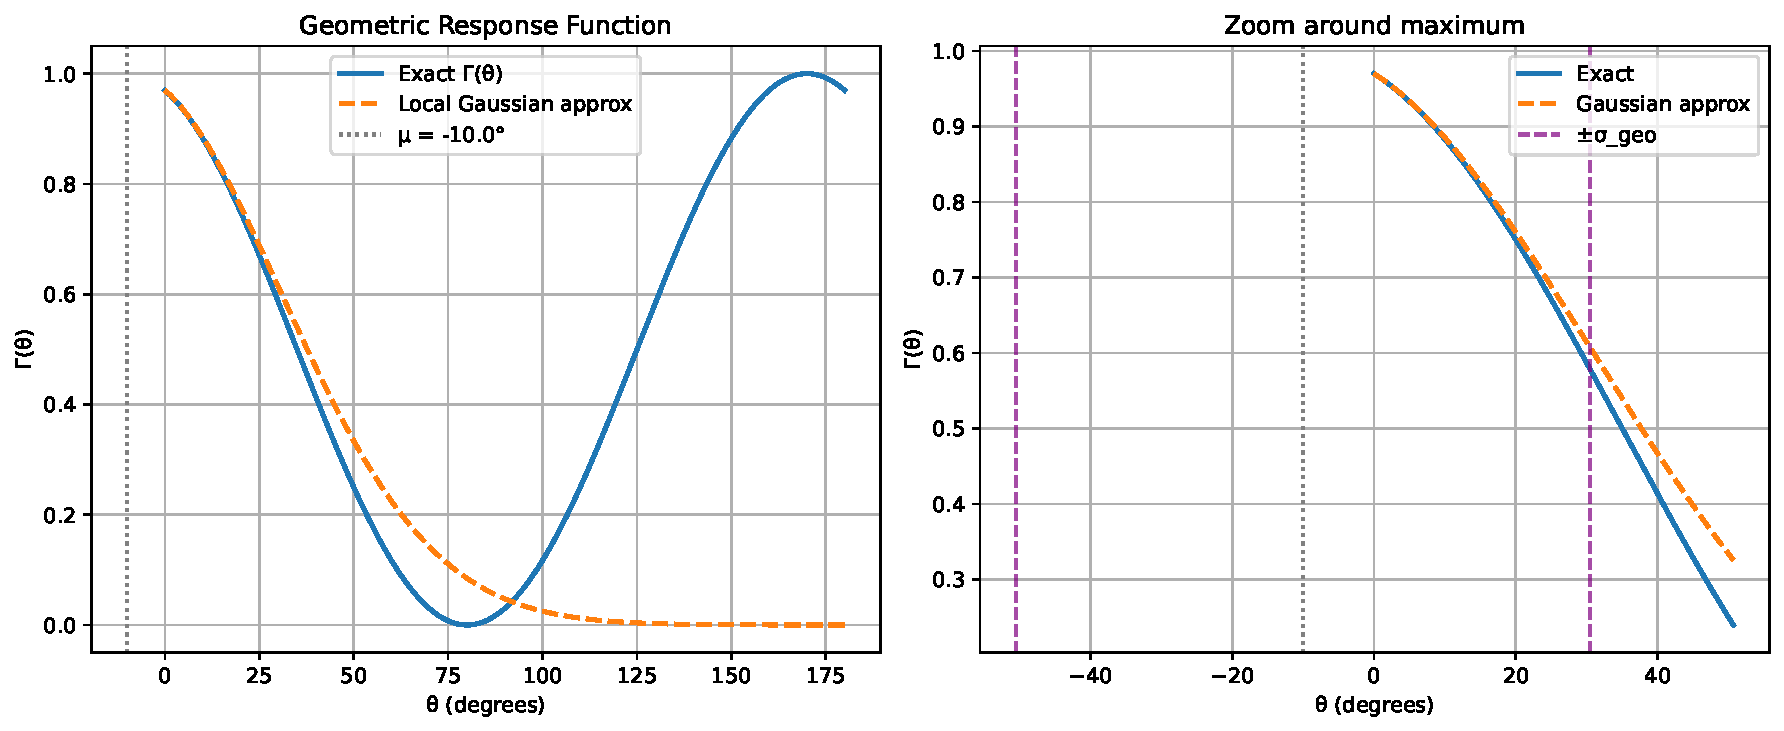
\includegraphics[width=\columnwidth]{figure_gamma.pdf}
\caption{The exact geometric response function
$\Gamma(\theta)=L^2\cos^2(\theta-\mu)$ (solid) compared with the
curvature-matched local approximation
$L^2\exp[-(\theta-\mu)^2/(2\sigma_{\rm geo}^2)]$ (dashed), for the
representative state $|\psi\rangle=\cos(50^\circ)|0\rangle+\sin(50^\circ)|1\rangle$.
Left: full angular range, period $\pi$. Right: zoom to
$|\theta-\mu|\le1.5\,\sigma_{\rm geo}$, vertical lines at
$\mu\pm\sigma_{\rm geo}$.}
\label{fig:gamma}
\end{figure}

%================================================
\section{Local curvature and geometric angular scale}
\label{sec:curvature}

The derivatives of $\Gamma$ at its maximum are
\begin{equation}
\Gamma'(\mu)=0,\qquad \Gamma''(\mu)=-2L^2,\qquad \Gamma'''(\mu)=0.
\label{eq:derivs}
\end{equation}
A Gaussian $L^2\exp[-(\theta-\mu)^2/(2\sigma^2)]$ has the same
second-order Taylor expansion at $\theta=\mu$ if
$\sigma^2 = -\Gamma(\mu)/\Gamma''(\mu)$. We define the
\emph{curvature-derived angular scale}
\begin{equation}
\boxed{\sigma_{\rm geo}= \frac{1}{\sqrt{2}}\;\text{rad} \approx 40.5^\circ}.
\label{eq:sigma}
\end{equation}

\begin{remark}[Universality of $\sigma_{\rm geo}$]
\label{rem:universal}
Equation~\eqref{eq:sigma} depends on $L$, $e_x$, $e_z$, $\gamma$,
$\eta$, $\beta$, and $\omega_c$ only through their absence: the ratio
$-\Gamma(\mu)/\Gamma''(\mu)$ is fixed by the functional form
$\cos^2(\theta-\mu)$ alone, which in turn follows purely from
$A(\theta)$ being a linear combination of $\sigma_x$ and $\sigma_z$
with unit-norm coefficients. $\sigma_{\rm geo}$ is therefore not a
material property of any particular bath or state; it is a
\emph{geometric invariant of the coupling family}, and its
experimental value (Section~\ref{sec:exp}) is a test of the
functional form~\eqref{eq:Gammacos} itself, not of any fitted
parameter. This scale is \emph{not} the width of a Gaussian fit to
$\Gamma(\theta)$: it is the unique Gaussian whose second-order Taylor
expansion matches the cosine squared. The exact function decays more
slowly than the Gaussian away from the peak: at
$|\theta-\mu|=\sigma_{\rm geo}$, $\Gamma=\cos^2(1/\sqrt2)L^2\approx0.578\,L^2$,
while the Gaussian gives $e^{-1/2}L^2\approx0.607\,L^2$, a fourth-order
effect of about $5\%$ (Appendix~\ref{app:gausserror}) that grows
rapidly beyond $1.5\,\sigma_{\rm geo}$, as shown in
Fig.~\ref{fig:error}.
\end{remark}

\begin{figure}[htbp]
\centering
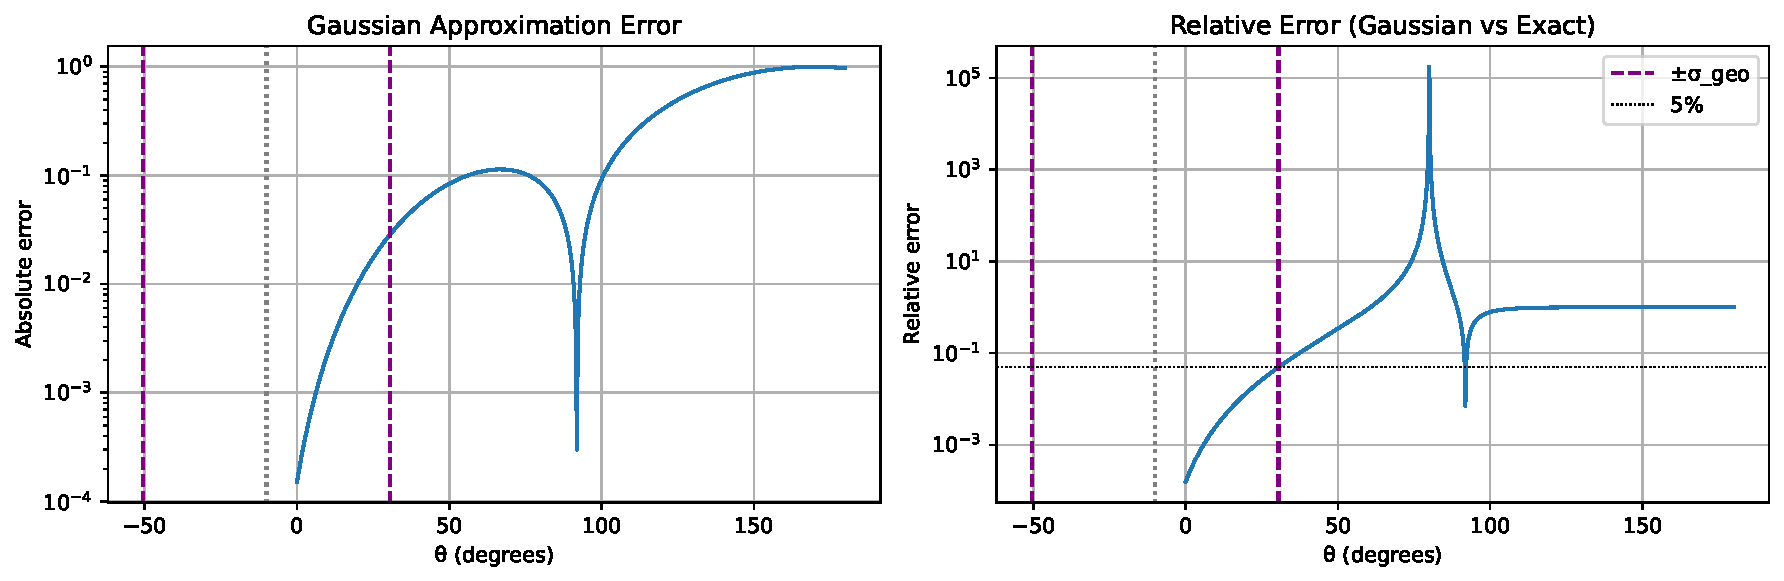
\includegraphics[width=\columnwidth]{figure_error.pdf}
\caption{Absolute (left) and relative (right) deviation between the
exact response $\Gamma(\theta)$ and its curvature-matched Gaussian
approximation, log scale, same reference state as Fig.~\ref{fig:gamma}.
The relative error stays below the $5\%$ line (horizontal dotted)
inside $|\theta-\mu|\le\sigma_{\rm geo}$ (vertical dashed) and grows
rapidly beyond it, confirming $\sigma_{\rm geo}$ delimits a strictly
local regime rather than a global fit.}
\label{fig:error}
\end{figure}

As shown in Fig.~\ref{fig:error} and quantified in
Appendix~\ref{app:gausserror}, this $5\%$ figure is itself a
parameter-free property of the $\cos^2$ functional form and would
apply identically to any two-level system realizing
Eq.~\eqref{eq:Gammacos}, regardless of the physical origin of the
coupling.

%================================================
\section{Time-dependent trajectories}
\label{sec:traj}

\subsection{Adiabatic-Markovian validity}
\label{sec:adiabatic}

The results above hold at fixed $\theta$. Suppose now that $\theta$ is
allowed to vary slowly in time, $\theta=\theta(t)$, so that
$H_S(t)\equiv H_S(\theta(t))=\omega_S A(\theta(t))$ and
$A(t)\equiv A(\theta(t))$ are now genuinely time-dependent operators
in the \emph{Schr\"odinger} picture -- a different, externally driven
time dependence from the interaction-picture constancy established in
Section~\ref{sec:model}, which held only at fixed $\theta$. Whether an
instantaneous generator $\mathcal L^{(D)}_{\theta(t)}$, built by simply
inserting $\theta(t)$ into Eq.~\eqref{eq:Lindblad}, provides a valid
description of the driven dynamics is not automatic and requires the
adiabatic-Markovian formalism of Albash \emph{et
al.}~\cite{albash2012adiabatic}, which established, from first
principles, the master equation appropriate to a system evolving
adiabatically while weakly coupled to a thermal bath. Two ingredients
of that formalism are favorable here. First, because $A(\theta)^2=I$
for every $\theta$, $H_S(\theta)=\omega_S A(\theta)$ has the
\emph{constant} spectral gap $2\omega_S$ for all $\theta$: unlike
generic adiabatic protocols, there is no risk of a closing gap
invalidating the adiabatic condition at some point along the
trajectory. Second, the bath correlation function is unaffected by
$\theta(t)$, so only the system side of the adiabatic condition needs
to be imposed. Adapting the standard adiabatic theorem together with
the time-scale separation of Section~\ref{sec:bath}, a sufficient
condition is
\begin{equation}
|\dot\theta| \ll \omega_S, \qquad
|\dot\theta| \ll \gamma, \qquad
|\dot\theta|\,\tau_B \ll 1,
\label{eq:adiahyp}
\end{equation}
i.e., the coupling angle must vary slowly compared to \emph{all three}
time scales of the problem: the (constant) system gap, the dissipative
rate, and the bath correlation time. Under
condition~\eqref{eq:adiahyp}, the instantaneous generator
$\mathcal L^{(D)}_{\theta(t)}$ of Eq.~\eqref{eq:Lindblad} provides a
controlled Markovian description at each instant. Unlike the previous
version of this section, we do not merely adapt
condition~\eqref{eq:adiahyp} by analogy: Appendix~\ref{app:rotating}
gives an exact change of frame, tracking the instantaneous eigenbasis
of $A(\theta(t))$, under which the naively-substituted generator is
shown to be the leading term of a controlled expansion in
$|\dot\theta|/\omega_S$, with the first condition in
Eq.~\eqref{eq:adiahyp} emerging from an explicit rotating-wave
argument rather than an assumed analogy; the coefficient of the
next-order correction is not computed there, only its parametric
suppression. This derivation supports \emph{only} the present
subsection -- none of Sections~\ref{sec:model}--\ref{sec:curvature},
nor the negative result of Section~\ref{sec:bridge} below, rely on it,
since those results are all obtained at fixed $\theta$ or from
Bloch-vector kinematics that hold regardless of the generator's precise
form. A separate condition
is needed to integrate it: Eq.~\eqref{eq:pureloss} is an initial rate,
derived for a pure state, and $|\psi(t)\rangle$ shrinks toward the
interior of the Bloch ball under Eq.~\eqref{eq:Lindblad} itself for
any $t>0$. Extrapolating the $t=0$ rate linearly,
\begin{equation}
\Delta P \approx 2\gamma\int_0^T
\bigl(\Gamma(\theta(t);\psi(0))-1\bigr)\,dt,
\label{eq:traj}
\end{equation}
is therefore only a \emph{leading-order} approximation, valid for
$|\Delta P|\ll\tfrac12$ (the full range available to a qubit), not for
arbitrary $T$. We verified this explicitly (Appendix~\ref{app:bloch}):
for the worst-case trajectory (maximal decay rate, $\Gamma\equiv0$),
Eq.~\eqref{eq:traj} agrees with the exact solution of the Bloch
equation to within $20\%$ for $\gamma T\lesssim0.2$, but becomes
unphysical -- predicting purity below the maximally-mixed floor of
$\tfrac12$ -- beyond $\gamma T\approx0.3$ (Fig.~\ref{fig:traj}). Using
Eq.~\eqref{eq:traj} beyond this regime requires solving the coupled
Bloch equation for $\mathbf r(t)$ directly rather than integrating the
initial rate. We stress that condition~\eqref{eq:adiahyp} and the
$|\Delta P|\ll\tfrac12$ condition just derived are two logically
independent requirements -- one on how fast $\theta(t)$ may vary, the
other on how long the linearized rate may be integrated -- and that
neither says anything about the relationship between $\Delta P$ and
any other trajectory functional, which we take up next.

\begin{figure}[htbp]
\centering
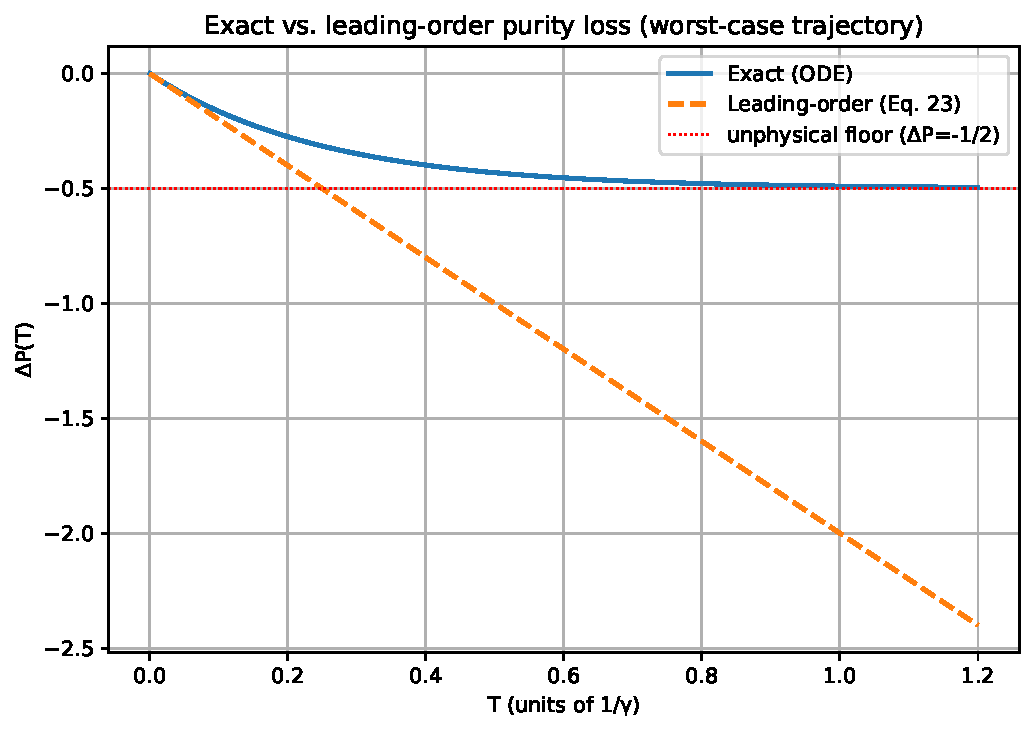
\includegraphics[width=\columnwidth]{figure_trajectory.pdf}
\caption{Exact purity loss (solving the Bloch equation) versus the
leading-order approximation of Eq.~\eqref{eq:traj}, for the worst-case
trajectory of Appendix~\ref{app:bloch} ($\Gamma\equiv0$, maximal decay
rate). The leading-order formula is accurate only for $\gamma
T\lesssim0.2$--$0.3$ and becomes unphysical (crosses the $\Delta
P=-1/2$ floor, dotted) beyond that.}
\label{fig:traj}
\end{figure}

\subsection{Relation to the biographical-witness functional}
\label{sec:bridge}

Reference~\cite{rodrigues2025} quantifies trajectory-dependent
decoherence through the Frobenius-norm functional
$\Wbio=\int_0^T\|\dot\rho(t)\|_F\,dt$, the arc length traced by the
density operator in the Hilbert--Schmidt metric, and reports
distinguishability between quantum twins via the Frobenius-norm
difference of their final states. It is tempting to identify
Eq.~\eqref{eq:traj} as a microscopic derivation of $\Wbio$; we show
here that this identification does \emph{not} hold in general, and we
isolate the obstruction explicitly rather than leave it implicit. The
argument below depends on none of the machinery of
Section~\ref{sec:adiabatic}: it uses only the general, model-independent
Bloch-vector identities~\eqref{eq:bloch}, which hold for \emph{any}
qubit dynamics, and is stated pointwise in time rather than as an
integrated trajectory quantity, so it is unaffected by whatever
remains open in the adiabatic reduction of Appendix~\ref{app:rotating}.

Write $\rho=(I+\mathbf r\cdot\boldsymbol\sigma)/2$ for a qubit. A short
calculation (Appendix~\ref{app:bloch}) gives, for \emph{any} qubit
dynamics,
\begin{equation}
\|\dot\rho\|_F = \frac{|\dot{\mathbf r}|}{\sqrt2},
\qquad
\frac{dP}{dt} = \mathbf r\cdot\dot{\mathbf r}.
\label{eq:bloch}
\end{equation}
The first quantity is the instantaneous \emph{speed} of the Bloch
vector; the second is its instantaneous \emph{radial} component of
motion (purity depends only on $|\mathbf r|$). These coincide only
when $\dot{\mathbf r}$ is parallel to $\mathbf r$ at every instant --
i.e., when the trajectory is a purely radial contraction with no
tangential (purity-preserving) component.

\begin{proposition}[Non-proportionality]
\label{prop:bridge}
$\Delta P$ [Eq.~\eqref{eq:traj}] is not proportional to $\Wbio$ in
general. This is a proven negative result, not an open question: the
two obstructions below establish it directly, one of which suffices.
\end{proposition}

\emph{Obstruction 1 (coherent contamination).} $\Wbio$ is defined in
Ref.~\cite{rodrigues2025} for arbitrary open-system trajectories, not
only commuting ones; testing it against a trajectory with a coherent
component is therefore squarely within its intended scope, even though
such a component falls outside the commuting restriction that defines
the microscopic model of Sections~\ref{sec:model}--\ref{sec:curvature}.
The Bloch-vector identities~\eqref{eq:bloch} used below hold for any
qubit dynamics, commuting or not. If the trajectory
includes any coherent (unitary) component -- for instance residual
precession from $H_S(\theta(t))$ itself, or any control imperfection
-- that component contributes to $|\dot{\mathbf r}|$, and hence to
$\Wbio$, while contributing \emph{exactly zero} to $dP/dt$, since
unitary evolution conserves purity. Concretely, for dephasing along a
fixed axis ($\theta=0$) with an added precession
$H_S=(\omega_0/2)\sigma_z$ -- which explicitly breaks
$[H_S,A]=0$, illustrating the general case rather than a property
internal to the commuting model -- acting on an equatorial state, one finds
$dP/dt=-2\gamma$ for \emph{every} value of $\omega_0$, while
$\|\dot\rho\|_F$ grows without bound as $\omega_0$ increases (a factor
of $25$ between $\omega_0=0$ and $\omega_0=50\gamma$ in the example
worked in Appendix~\ref{app:bloch}). $\Wbio$ is therefore sensitive to
coherent dynamics that $\Delta P$ cannot see at all.

\emph{Obstruction 2 (linear vs.\ quadratic dependence).} Even in the
strictly dissipative sub-case with no coherent term at all, and with
the Bloch vector confined to the plane transverse to the coupling axis
($\mathbf r=\mathbf r_\perp$, purely radial decay, $\dot{\mathbf
r}=-2\gamma\mathbf r_\perp$), Eq.~\eqref{eq:bloch} gives
\begin{equation}
\|\dot\rho\|_F = \sqrt2\,\gamma\,|\mathbf r_\perp|,
\qquad
\frac{dP}{dt} = -2\gamma\,|\mathbf r_\perp|^2 ,
\end{equation}
linear and quadratic in $|\mathbf r_\perp|$, respectively
(Appendix~\ref{app:bloch}). Their ratio is $-\sqrt2\,|\mathbf r_\perp|$,
which is not constant along a trajectory on which $|\mathbf r_\perp|$
itself decays. So even in the most favorable case -- no coherent
term, and motion restricted to the purely radial direction -- $\Wbio$
and $\Delta P$ are related by a state-dependent, nonlinear map, not a
proportionality constant.

We conclude that Eq.~\eqref{eq:traj} is a rigorous microscopic result
for the purity-loss functional in its own right, and it is
\emph{consistent with} the qualitative claim of
Ref.~\cite{rodrigues2025} that trajectory geometry affects decoherence
outcomes, but it does not constitute a derivation of $\Wbio$ or of the
phenomenological relation between decoherence strength and trajectory
length proposed there.

\begin{openproblem}
\label{op:bridge}
Proposition~\ref{prop:bridge} rules out the naive identification
$\Delta P\propto\Wbio$; it does not rule out every possible relation.
Is there a restriction of $\Wbio$ (e.g., to its radial component) or a
reformulation of the phenomenological model of
Ref.~\cite{rodrigues2025} directly in terms of $\Gamma(\theta(t))$
under which a well-defined, non-trivial relation to the present
microscopic results can be established?
\end{openproblem}

%================================================
\section{Experimental feasibility}
\label{sec:exp}

The static and dynamic results of this paper require different
experimental platforms, and conflating them would overstate what a
single setup can test. We treat them separately.

\subsection{Static-angle predictions (linear optics)}
\label{sec:exp_static}

The predictions below concern the coupling-angle dependence of
Sections~\ref{sec:response}--\ref{sec:curvature} at fixed $\theta$,
which does not require the adiabatic machinery of
Section~\ref{sec:traj}.

\begin{enumerate}
\item \textbf{Peak direction.} For any prepared pure state, the
coupling angle of minimum purity loss must be
$\mu=\operatorname{atan2}(e_z,e_x)$; varying the initial state tests
this relation directly.
\item \textbf{Angular profile.} The purity-loss rate must follow
$\cos^2(\theta-\mu)$, with curvature ratio $\Gamma''(\mu)/\Gamma(\mu)=-2$
(Remark~\ref{rem:universal}), independent of state, temperature, and
coupling strength.
\item \textbf{Minimum.} The minimum of $\Gamma$ occurs at $\mu+\pi/2$.
\end{enumerate}

A natural platform is a photonic polarization qubit, with $\theta$ set
by a wave-plate angle and a controllable dephasing channel implemented
interferometrically -- e.g., a displaced Sagnac interferometer of the
kind already used to engineer amplitude-damping and dephasing channels
on polarization qubits under waveplate control in weak-measurement and
measurement-reversal experiments. A wave plate applies a fixed,
essentially instantaneous unitary at a localized point in the optical
path; this is entirely adequate for setting a \emph{constant} $\theta$
per run and scanning it across runs, which is all predictions 1--3
require.

Two quantitative constraints from the microscopic theory bound the
feasible parameter regime. First, Section~\ref{sec:bath} requires the
system evolution (interrogation) time to satisfy $t\gtrsim10$--$50\,\tau_B$
for the Markov truncation error to fall in the few-percent range
(Table~\ref{tab:tail}); for an engineered interferometric bath, $\tau_B$
is set by the interferometer's own delay and is therefore, unlike a
solid-state phonon bath, a design parameter that can be made short
compared to the achievable interrogation time. Second, resolving the
$5\%$ deviation between $\Gamma(\theta)$ and its Gaussian approximation
(Remark~\ref{rem:universal}) at $\theta=\mu\pm\sigma_{\rm geo}$ requires
angular control and readout precision below this level; motorized
wave-plate stages with sub-degree repeatability, already standard in
polarization-qubit process tomography, are more than adequate, since
$\sigma_{\rm geo}\approx40.5^\circ$ is a coarse angular scale on that
scale. We do not attempt a full experimental design here; the point is
that the constraints imposed by Sections~\ref{sec:bath}
and~\ref{sec:curvature} are quantitative and platform-independent, and
should be checked explicitly against any specific realization rather
than assumed.

\subsection{Dynamic/trajectory predictions: a different platform is needed}
\label{sec:exp_dynamic}

The adiabatic-Markovian regime of Section~\ref{sec:traj} requires
$\theta(t)$ to vary \emph{continuously in time while the dissipative
generator acts concurrently}, on the time scales set by
condition~\eqref{eq:adiahyp}. A single wave plate in a linear-optical,
single-pass architecture does not realize this: it is a localized,
essentially instantaneous gate per photon, not a continuously driven
Hamiltonian $H_S(\theta(t))$ acting in parallel with an open-system
bath over an extended interrogation window. Reference~\cite{rodrigues2025}
proposes a photonic protocol for its own trajectory-dependent effect,
which is not, on the same grounds, obviously compatible with a static
per-photon wave-plate setting either; we do not assume here that it
resolves this mismatch, and we do not claim that the static platform
of Section~\ref{sec:exp_static} tests the dynamic content of
Section~\ref{sec:traj}. Testing the adiabatic regime and
Open~Problem~\ref{op:bridge} directly calls for a platform with
genuine continuous-time Hamiltonian control concurrent with
dissipation -- for instance a driven superconducting qubit or an NV
center, where $\theta(t)$ could be realized as a continuously
modulated control field -- which we leave to future work rather than
retrofit onto the static proposal above.

%================================================
\section{Discussion}
\label{sec:discussion}

We have derived, from a microscopic model with commuting qubit--bath
coupling, an exact relation between the initial purity-loss rate and
the geometric overlap $\Gamma(\theta)$, with the angle-independence of
the dissipative generator's norm (Theorem~\ref{thm:norm}) now
established in closed form rather than by numerical search alone. The
cosine-squared form and the curvature scale $1/\sqrt2$ are universal
within this coupling family (Remark~\ref{rem:universal}).

This work does not claim to derive trajectory dependence in full
generality, nor -- see Section~\ref{sec:bridge} -- does it claim to
derive the phenomenological witness of Ref.~\cite{rodrigues2025} from
first principles; it isolates a minimal, exactly solvable setting in
which the angular mechanism available to any such model can be made
precise, and it identifies specifically where a bridge to the
phenomenological model would need to be built. When the coupling
operator is externally varied, the effective decoherence naturally
becomes history-dependent; this is consistent with the process-tensor
framework~\cite{pollock2018nonmarkovian,milz2021quantum} and with the
broader literature on non-Markovian quantum
dynamics~\cite{rivas2014quantum,devega2017dynamics,breuer2009measure}.

We note explicitly that $\Gamma(\theta)$ is \emph{not} an instance of
the geometric (Berry) phase acquired by an adiabatically evolving open
system, a distinct and more established notion of ``geometric''
decoherence in which a slowly cycled Hamiltonian parameter picks up a
holonomy corrected by the
bath~\cite{dechiara2003berry}; nor is it a Loschmidt-echo-type fidelity
susceptibility to a Hamiltonian
perturbation~\cite{cucchietti2003decoherence}. $\Gamma(\theta)$ is
simply the squared overlap of a fixed reference state with the
coupling operator itself, evaluated at fixed $\theta$; the word
``geometric'' here refers only to this overlap structure on the Bloch
sphere, not to a holonomy or a topological invariant. The bath
correlation function used in Section~\ref{sec:bath}, and the resulting
pure-dephasing rate $\gamma$, are also the objects of the filter-function
and noise-spectroscopy formalism used to characterize and mitigate
qubit dephasing experimentally~\cite{cywinski2008enhance}; realized
dephasing times well in excess of $100\,\mu$s alongside $T_1\sim
10\,\mu$s have been demonstrated for a driven superconducting qubit
using exactly this class of
technique~\cite{bylander2011noise}, which is the concrete precedent
behind the solid-state platform proposed for the dynamic regime in
Section~\ref{sec:exp}.

The restriction to a commuting interaction (Remark~\ref{rem:HS_choice})
limits the immediate applicability of the exact results of
Sections~\ref{sec:generator}--\ref{sec:curvature}: they hold only so
long as the system's free-evolution axis remains locked to the
coupling geometry. We have not verified that this alignment survives
under generic extensions of the model -- for instance, additional
qubits, additional coupling channels, or coupling operators that are
not simple linear combinations of two Pauli matrices -- and we
explicitly flag this as untested rather than assumed to generalize.
The geometric structure identified here (a $\cos^2$ response with a
universal, parameter-free curvature scale) is a feature of the
two-dimensional coupling family~\eqref{eq:Atheta} specifically; a
non-commuting or higher-dimensional extension would need to be
re-derived, likely under a secular approximation, and there is no
guarantee that the same closed forms survive that step.

Future work should extend the analysis to non-commuting couplings and
to mixed initial states, address Open Problem~\ref{op:bridge}, and
examine the connection with process-tensor-based measures of
non-Markovianity.

%================================================
\section{Conclusion}
\label{sec:conclusion}

For a qubit coupled to a thermal Ohmic bath through a commuting
interaction $A(\theta)$, the state-resolved purity-loss rate exhibits
an exact $\cos^2(\theta-\mu)$ dependence, and the norm of the
Born--Markov dissipative generator is provably constant in $\theta$
(Theorem~\ref{thm:norm}), isolating the geometric origin of the
angular modulation. The curvature-defined angular scale
$\sigma_{\rm geo}=1/\sqrt2$ is a universal, parameter-free invariant of
the coupling family. The Markov approximation underlying these results
converges only algebraically (Proposition~\ref{prop:tail}), a
quantitative constraint on any proposed realization. A slowly varying
coupling angle admits a well-defined adiabatic-Markovian generator,
but we prove that its integrated purity loss does not, in
general, coincide with the trajectory-integrated Frobenius-norm
witness of the phenomenological model it was meant to underwrite
(Proposition~\ref{prop:bridge}); whether any restricted or
reformulated version of that witness does is stated as an explicit,
narrower open problem rather than papered over. The results
above stand on their own as an exact microscopic benchmark for
state-resolved, angle-dependent decoherence, independent of that
open problem's resolution.

\begin{acknowledgments}
The author acknowledges the foundational contributions of the
Nakajima--Zwanzig formalism, the weak-coupling-limit derivations of
Davies and of D\"umcke and Spohn, and the process-tensor framework.
Symbolic and numerical verifications were performed with SymPy,
NumPy, and SciPy.
\end{acknowledgments}

%================================================
\appendix

\section{Explicit Nakajima--Zwanzig to Markov reduction}
\label{app:NZ}

This appendix makes explicit the steps compressed into
Eqs.~\eqref{eq:NZ}--\eqref{eq:gamma}.

\emph{Step 1 (projectors).} Define $\mathcal{P}X=\tr_B(X)\otimes\rho_B$
and $\mathcal{Q}=\mathcal{I}-\mathcal{P}$. The exact reduced dynamics
obeys the Nakajima--Zwanzig equation
\begin{align}
\dot\rho(t) &= -i\tr_B[H_I(t),\rho_{\rm tot}(t)]
-\int_0^t ds\,\tr_B\Bigl[H_I(t),\notag\\
&\qquad
e^{(t-s)\mathcal{QL}}\mathcal{QL}[H_I(s),\rho(s)\otimes\rho_B]\Bigr],
\end{align}
where $\mathcal{L}X=-i[H_{\rm tot},X]$. The first term vanishes
because $\tr_B[A(\theta),\rho_B B]=A(\theta)\rho\,\tr_B(\rho_B B)=0$
for a thermal bath ($\langle B\rangle_{\rho_B}=0$).

\emph{Step 2 (Born approximation).} To second order in $H_I$, replace
$e^{(t-s)\mathcal{QL}}\to e^{(t-s)\mathcal{L}_B}$ (free bath
propagation) and $\rho(s)\to\rho(t)$ (slowly varying system, valid for
$\tau_B\ll\tau_S$; see Section~\ref{sec:bath} for the quantitative
version of this condition). This gives Eq.~\eqref{eq:NZ}.

\emph{Step 3 (commuting interaction picture).} Because
$[H_S(\theta),A(\theta)]=0$ (Eq.~\eqref{eq:comm}), the
interaction-picture coupling operator is time-independent,
$A_I(t)=A(\theta)$. Only the bath operator carries time dependence.
Expanding the double commutator and tracing over the bath using
$\tr_B[\rho_B B(0)B(s)]=C(s)$ yields Eq.~\eqref{eq:kernel}.

\emph{Step 4 (Markov limit).} Since
$\int_0^\infty|C(s)|\,ds=\pi\eta/\beta<\infty$ (Eq.~\eqref{eq:intC}),
the upper limit is extended to infinity with the error quantified in
Proposition~\ref{prop:tail} and Table~\ref{tab:tail}. Using $A^2=I$,
$[A,[A,\rho]]=2(\rho-A\rho A)$, giving the time-independent Lindblad
generator of Eqs.~\eqref{eq:Lindblad}--\eqref{eq:gamma}. No secular
approximation is required at any step, because Eq.~\eqref{eq:comm}
guarantees a single time-independent coupling operator throughout;
this is the structural simplification purchased by the
commuting-coupling restriction (Remark~\ref{rem:HS_choice}).

\section{Rotating-frame derivation of the adiabatic condition}
\label{app:rotating}

This appendix derives condition~\eqref{eq:adiahyp} rather than
assuming it by analogy, for the specific case of Section~\ref{sec:traj}.
It supports only that section; it is not used elsewhere.

\emph{Exact change of frame.} Let $V(t)=e^{i\theta(t)\sigma_y/2}$,
which satisfies $V^\dagger A(\theta(t))V=\sigma_x$ for every $t$ (a
direct consequence of $A(\theta)$ being confined to the $xz$-plane,
verified symbolically). Define $\tilde\rho(t)=V(t)^\dagger\rho(t)V(t)$.
Since $V^\dagger\dot V=i\dot\theta\sigma_y/2$ and
$\dot V^\dagger V=-i\dot\theta\sigma_y/2$, the product rule gives,
\emph{exactly} (no approximation yet),
\begin{equation}
\dot{\tilde\rho} = -i\bigl[\omega_S\sigma_x+\tfrac{\dot\theta}{2}\sigma_y,\,\tilde\rho\bigr]
+\gamma\bigl(\sigma_x\tilde\rho\sigma_x-\tilde\rho\bigr),
\label{eq:rotframe}
\end{equation}
starting from the naively-substituted lab-frame equation
$\dot\rho=-i[H_S(\theta(t)),\rho]+\mathcal L^{(D)}_{\theta(t)}[\rho]$
(both sides were checked to agree identically with SymPy, for a
general $\rho$, before writing this). Equation~\eqref{eq:rotframe}
shows that in this frame the dissipator is the fixed, $\theta$-independent
$\sigma_x$-dephasing generator of Sections~\ref{sec:generator}--\ref{sec:norm}
for \emph{every} trajectory $\theta(t)$: all of the time-dependence has
been moved into a single extra coherent term, $(\dot\theta/2)\sigma_y$,
which is exactly the obstruction, since
$[\sigma_x,\sigma_y]=2i\sigma_z\neq0$: it is this term, and only this
term, that reintroduces the non-commuting structure the rest of the
paper is built to avoid.

\emph{Why $|\dot\theta|\ll\omega_S$ suppresses it.} In the interaction
picture with respect to the dominant part $\omega_S\sigma_x$,
\begin{align}
\sigma_y(\tau) &= e^{i\omega_S\sigma_x\tau}\sigma_y e^{-i\omega_S\sigma_x\tau}\notag\\
&= \cos(2\omega_S\tau)\,\sigma_y - \sin(2\omega_S\tau)\,\sigma_z,
\end{align}
verified symbolically, i.e., the extra term oscillates at the
\emph{constant} gap frequency $2\omega_S$ and averages to zero over
any window long compared to $1/\omega_S$ but short compared to the
timescale $1/|\dot\theta|$ over which its prefactor changes. This is
exactly the standard rotating-wave argument, now applied to the extra
term rather than to the dephasing structure itself, and it is precisely
what requires $|\dot\theta|\ll\omega_S$: the prefactor must vary slowly
compared to the oscillation it multiplies. Under this condition, the
extra term's leading effect on the coarse-grained (Markovian) dynamics
of $\tilde\rho$ averages away, recovering
Eq.~\eqref{eq:Lindblad}$|_{\theta\to\theta(t)}$ as the leading-order
result. We have not computed the coefficient of the next-order
correction (organized in powers of $|\dot\theta|/\omega_S$), only
demonstrated the mechanism that suppresses it and the parameter it is
suppressed by; the two remaining conditions in
Eq.~\eqref{eq:adiahyp} continue to be adapted by analogy with the
Markov and bath-memory constraints of Section~\ref{sec:bath}, not
independently rederived here.

\section{Purity decay formula}
\label{app:purity}

Derivation of Eq.~\eqref{eq:pureloss}: using
Eq.~\eqref{eq:Lindblad} and $A^2=I$,
\begin{align}
\tr(\rho\mathcal{L}^{(D)}_\theta[\rho])
&= \gamma\tr(\rho A\rho A - \rho^2) \nonumber\\
&= \gamma\bigl(|\langle\psi|A|\psi\rangle|^2 - 1\bigr),
\end{align}
where the last step uses $\rho=|\psi\rangle\langle\psi|$, so
$\tr(\rho A\rho A)=\langle\psi|A|\psi\rangle\langle\psi|A|\psi\rangle
=|\langle\psi|A|\psi\rangle|^2$. In the eigenbasis of $A(\theta)$
(eigenvalues $\pm1$), writing $\rho$ with entries $\rho_{ij}$, one has
$A\rho A-\rho=\mathrm{diag}(0,0)$ off the diagonal replaced by
$-2\rho_{01},-2\rho_{10}$: populations are unaffected and only
coherences decay, confirming the pure-dephasing character of the
model stated in Section~\ref{sec:model}.

\section{Algebraic Markov tail: closed form}
\label{app:tail}

The symbolic tail integral used for Proposition~\ref{prop:tail} and
Table~\ref{tab:tail}, verified with SymPy, is
\begin{align}
\int_t^\infty C(s)\,ds
&= \frac{2\eta\omega_c}{\beta}\int_t^\infty\frac{ds}{1+\omega_c^2s^2}\notag\\
&= \frac{\eta}{\beta}\Bigl[\pi-2\arctan(\omega_c t)\Bigr].
\end{align}
Using $\arctan(x)=\pi/2-1/x+O(x^{-3})$ for large $x$ gives the
algebraic large-$t$ behavior quoted in Eq.~\eqref{eq:tail}. The
numerical values in Table~\ref{tab:tail} follow by dividing by
$\int_0^\infty C\,ds=\pi\eta/\beta$ and setting $\eta=\beta=\omega_c=1$.

\section{Local Gaussian approximation error}
\label{app:gausserror}

Expanding $\cos^2 x = 1 - x^2 + \frac{x^4}{3} + O(x^6)$ and
$e^{-x^2} = 1 - x^2 + \frac{x^4}{2} + O(x^6)$, the difference is
$-\frac{x^4}{6} + O(x^6)$. At $x=\sigma_{\rm geo}=1/\sqrt{2}$, the
absolute difference (from the full, non-truncated expressions, as
computed by the reproducibility script) is $\approx0.0286$. This
figure is reported here relative to two different quantities, which
must not be conflated: relative to the \emph{local} exact value at
that point, $\Gamma(\mu+\sigma_{\rm geo})\approx0.578\,L^2$, it is
$\approx4.95\%$; relative to the \emph{peak} value $\Gamma(\mu)=L^2$,
it is $\approx2.86\%$. Both are printed explicitly, and labeled, by
the reproducibility script; the main text (Remark~\ref{rem:universal})
and Fig.~\ref{fig:error} use the local figure, since that is the
relevant one for judging the accuracy of the Gaussian approximation
\emph{at} the point being evaluated, not relative to a different point
(the peak) on the curve.

\section{Bloch-vector calculations for Section~\ref{sec:bridge}}
\label{app:bloch}

For $\rho=(I+\mathbf r\cdot\boldsymbol\sigma)/2$,
$\dot\rho=(\dot{\mathbf r}\cdot\boldsymbol\sigma)/2$. Since
$\tr(\sigma_i\sigma_j)=2\delta_{ij}$,
$\|\dot\rho\|_F^2=\tr(\dot\rho^2)=\tfrac14\tr[(\dot{\mathbf r}\cdot\boldsymbol\sigma)^2]
=\tfrac14(2|\dot{\mathbf r}|^2)=|\dot{\mathbf r}|^2/2$, giving the
first identity in Eq.~\eqref{eq:bloch}. Purity is
$P=\tr(\rho^2)=(1+|\mathbf r|^2)/2$, so $dP/dt=\mathbf r\cdot\dot{\mathbf r}$,
the second identity.

\emph{Obstruction 1, worked example.} Take $\theta=0$ ($A=\sigma_x$,
dephasing preserves the $x$-component) with
$H_S=(\omega_0/2)\sigma_z$ added. The Bloch equations are
$\dot r_x=-\omega_0 r_y$, $\dot r_y=\omega_0 r_x-2\gamma r_y$,
$\dot r_z=-2\gamma r_z$. At the equatorial state $\mathbf r=(0,1,0)$,
$\dot{\mathbf r}=(-\omega_0,-2\gamma,0)$, so
$dP/dt=\mathbf r\cdot\dot{\mathbf r}=-2\gamma$ for every $\omega_0$,
while $\|\dot\rho\|_F=\sqrt{(\omega_0^2+4\gamma^2)/2}$ grows without
bound. Numerically, $\|\dot\rho\|_F/\gamma\approx1.41,\,1.58,\,7.21,\,35.4$
at $\omega_0/\gamma=0,1,10,50$, respectively, while $dP/dt=-2\gamma$
throughout.

\emph{Obstruction 2, worked example.} For purely radial decay
($\mathbf r=\mathbf r_\perp$, $\dot{\mathbf r}=-2\gamma\mathbf r_\perp$),
Eq.~\eqref{eq:bloch} gives $\|\dot\rho\|_F=\sqrt2\,\gamma|\mathbf r_\perp|$
and $dP/dt=-2\gamma|\mathbf r_\perp|^2$ directly by substitution.

\emph{Eq.~\eqref{eq:traj}, worst-case worked example.} Take $\theta=0$
fixed ($\mathbf n=\hat{\mathbf x}$) and the initial state
$\mathbf r(0)=(0,1,0)$, so $\Gamma(0)=0$ throughout (the
$\hat{\mathbf x}$-component of $\mathbf r$ never changes at fixed
$\theta$, and starts at zero): this is the maximal-decay-rate case,
the fastest that $\Delta P$ can accumulate for this model. The exact
Bloch equation $\dot{\mathbf r}=\gamma(R_0-I)\mathbf r$ integrates in
closed form, $\mathbf r_\perp(t)=\mathbf r_\perp(0)e^{-2\gamma t}$,
giving $\Delta P_{\rm exact}(T)=\bigl(e^{-4\gamma T}-1\bigr)/2$, while
Eq.~\eqref{eq:traj} gives $\Delta P_{\rm naive}(T)=-2\gamma T$ (using
$\Gamma\equiv0$). Table~\ref{tab:traj} compares the two (values from
the reproducibility script, direct ODE integration, $\gamma=1$).

\begin{table}[htbp]
\centering
\caption{Exact vs.\ leading-order [Eq.~\eqref{eq:traj}] purity loss for
the worst-case trajectory of this appendix. Eq.~\eqref{eq:traj} is
unphysical ($\Delta P<-1/2$) beyond $\gamma T\approx0.3$.}
\label{tab:traj}
\begin{tabular}{ccc}
\hline\hline
$\gamma T$ & $\Delta P_{\rm exact}$ & $\Delta P_{\rm naive}$ (Eq.~\eqref{eq:traj}) \\
\hline
0.05 & $-0.091$ & $-0.100$ \\
0.10 & $-0.165$ & $-0.200$ \\
0.20 & $-0.275$ & $-0.400$ \\
0.30 & $-0.349$ & $-0.600$ (unphysical) \\
0.50 & $-0.432$ & $-1.000$ (unphysical) \\
\hline\hline
\end{tabular}
\end{table}

\section{Numerical cross-checks of Theorem~\ref{thm:norm}}
\label{app:numcheck}

The reproducibility script performs two independent numerical checks,
neither of which is the primary evidence for Theorem~\ref{thm:norm}
(the closed-form proof in Section~\ref{sec:norm} is). First, exact
evaluation of $\|\mathcal L^{(D)}_\theta[X]\|_1/\|X\|_1$ on the three
basis operators $\{\sigma_x,\sigma_y,\sigma_z\}$ of $\mathcal B_0$, at
nine values of $\theta\in[0,\pi]$. This is not, in general, sufficient
to find the maximum of a quadratic-form ratio over $\mathcal B_0$ --
extrema of such ratios are generally attained only on the eigenbasis of
the associated operator, not on an arbitrary spanning set. It is
sufficient \emph{here} for a structural reason specific to this
coupling family: since $\mathbf n_\theta=(\cos\theta,0,\sin\theta)$
has zero $y$-component for every $\theta$ (Eq.~\eqref{eq:Atheta}
involves only $\sigma_x,\sigma_z$), $\hat{\mathbf y}$ is orthogonal to
$\mathbf n_\theta$ for every $\theta$, and by Lemma~\ref{lem:eigenvalues}
the $2$-dimensional eigenspace of $R_\theta-I$ with the maximal
eigenvalue $-2$ is exactly the plane orthogonal to $\mathbf n_\theta$.
Hence $\sigma_y$ alone is guaranteed to lie in that maximal eigenspace
for every $\theta$, and evaluating on it already attains the exact
supremum; $\sigma_x,\sigma_z$ are included only for redundancy. This
argument is specific to a coupling family confined to the $xz$-plane
and would need to be redone -- most directly, by evaluating on the
actual eigenbasis of $R_\theta-I$ rather than on a fixed
$\theta$-independent triple -- for any extension in which
$\mathbf n_\theta$ acquires a $y$-component; all $27$ evaluations
reproduce $2\gamma$ to
$10^{-10}$ relative precision. Second, as a further, method-independent
check, a global numerical search for $\sup_X\|\mathcal
L^{(D)}_\theta[X]\|_1/\|X\|_1$ over $\mathbf r\in S^2$, at the same
nine angles, using Nelder--Mead with $20$ random restarts per angle
(tolerance $10^{-12}$): all nine maxima agree with $2\gamma$ to within
$10^{-8}$ relative precision. Both are consistent with, and logically
subordinate to, the closed-form result of Theorem~\ref{thm:norm}.

%================================================

\bibliography{references}

\end{document}
